\documentclass{genrel}

\makeindex

\begin{document}

\thispagestyle{empty}
\raisebox{0mm}[0mm][0mm]{%
\parbox{8.5in}{
\vspace*{236mm}\hspace{-38.5mm}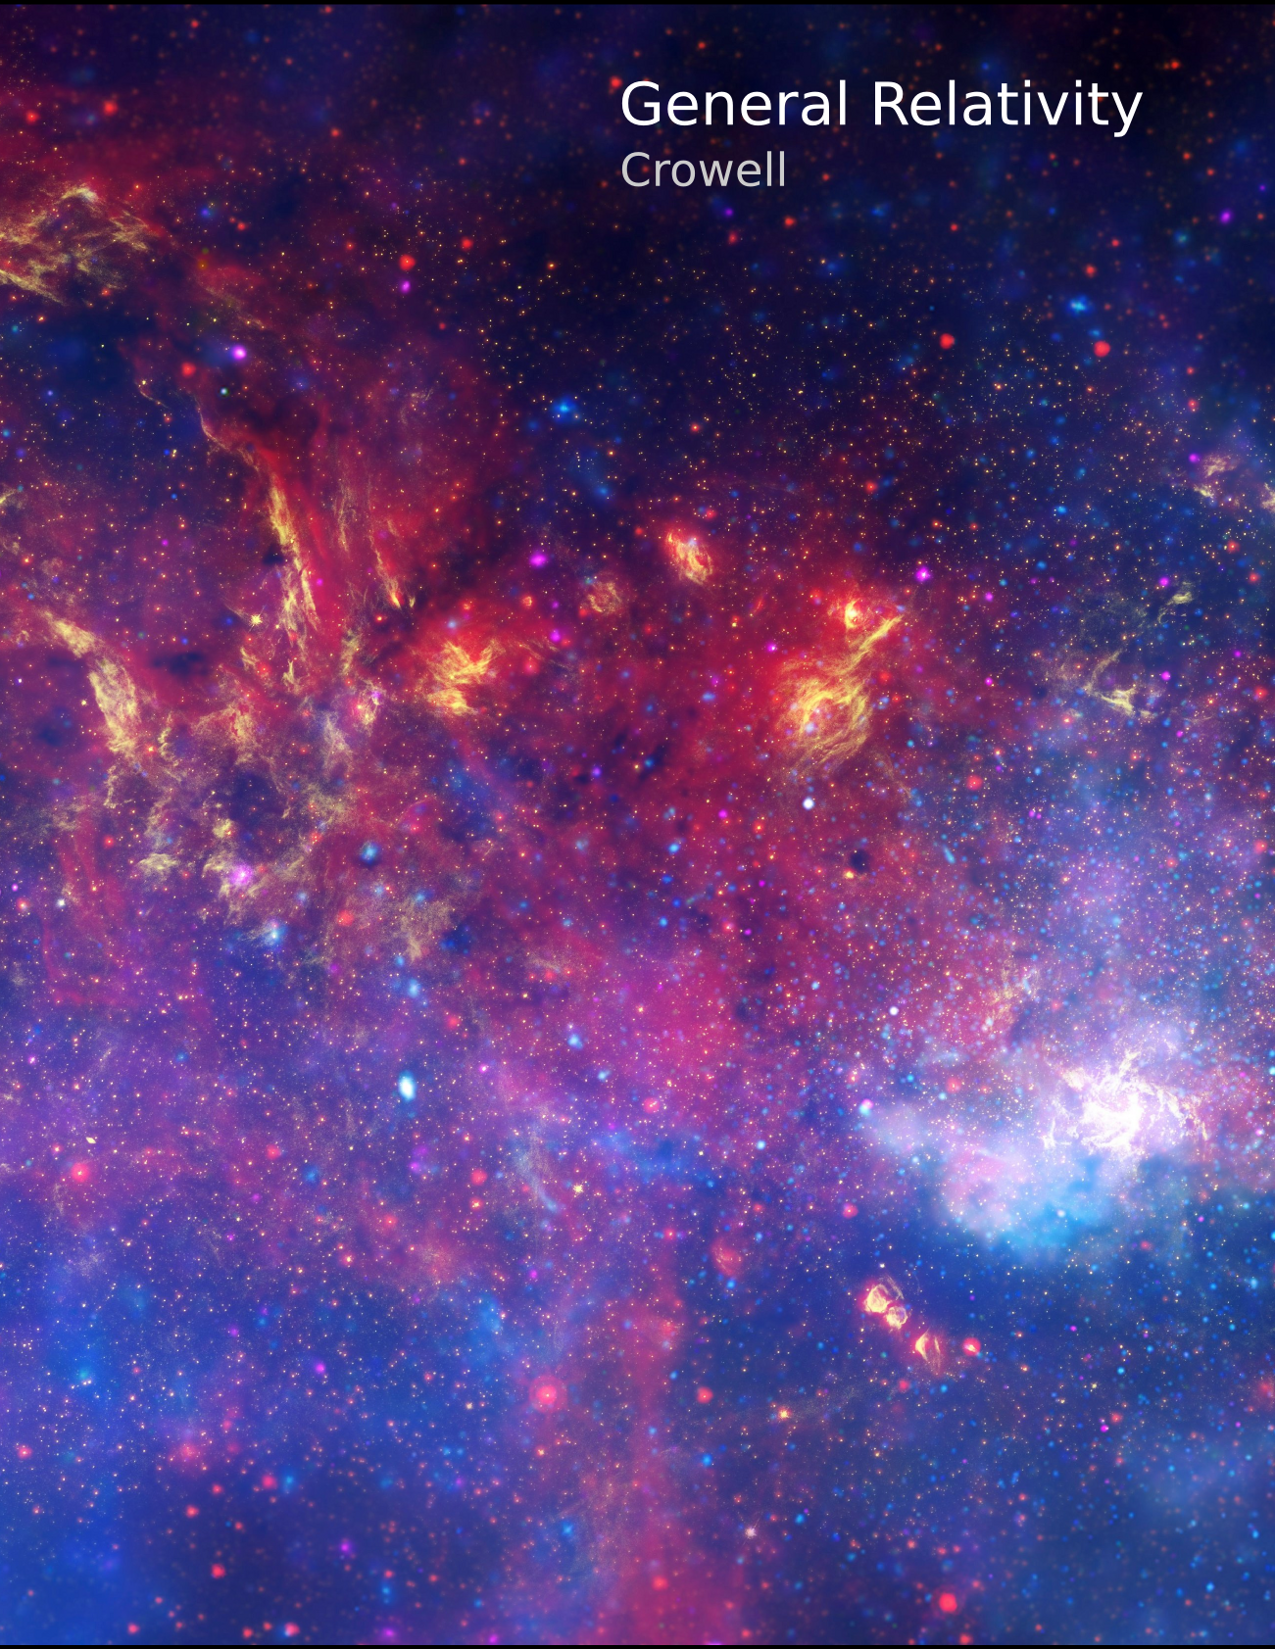
\includegraphics{cover/cover-for-pdf.png}\\
}
}%
\\


\cleardoublepage

\thispagestyle{empty}

\vspace{100mm}

{\sffamily

\noindent {\Huge General Relativity}

\noindent Benjamin Crowell

\noindent www.lightandmatter.com

}


\thispagestyle{empty}

\vspace{100mm}

\noindent
\includegraphics{cover/lmlogo}\\
Fullerton, California\\
www.lightandmatter.com

\vspace{20mm}
\noindent
Copyright \copyright  2009 Benjamin Crowell

\vspace{20mm}
\noindent
rev. \today{}

\vspace{6mm}
\noindent
Permission is granted to copy, distribute and/or modify this
document under the terms of the Creative Commons Attribution
Share-Alike License, which can be found at creativecommons.org. The license
applies to the entire text of this book, plus all the illustrations
that are by Benjamin Crowell. All the illustrations are by Benjamin
Crowell except as noted in the photo credits or in parentheses
in the caption of the figure.
This book can be downloaded free of charge
from www.lightandmatter.com in a variety of formats,
including editable formats.


\pagebreak\vspace{100mm}

\hbox{}\noindent\huge\bfseries\sffamily{}\hspace{-2mm}\ \ Brief Contents\\
\hspace{-20mm}\noindent\mynormaltype\Large\sffamily{}\begin{tabular}{rl}
\ref{ch:intro} & A Geometrical Theory of Spacetime \quad \pageref{ch:intro}\\
\ref{ch:flat} & Geometry of Flat Spacetime \quad \pageref{ch:flat}\\
\ref{ch:differential-geometry} & Differential Geometry \quad \pageref{ch:differential-geometry}\\
\ref{ch:tensors} & Tensors \quad \pageref{ch:tensors}\\
\ref{ch:curvature} & Curvature \quad \pageref{ch:curvature}\\
\ref{ch:vacuum} & Vacuum Solutions \quad \pageref{ch:vacuum}\\
\ref{ch:sources} & Sources \quad \pageref{ch:sources}\\
\ref{ch:waves} & Gravitational Waves \quad \pageref{ch:waves}\\
\end{tabular}
\mynormaltype

\vspace{100mm}\pagebreak

\cleardoublepage

\noindent\huge\bfseries\sffamily{}\hspace{-2mm}\ \ Contents\\
\mynormaltype

\tableofcontents

%========================= main matter =========================
\mainmatter
%-- I want the whole book numbered sequentially, arabic:
  \pagenumbering{arabic} 
  \addtocounter{page}{10} 
\parafmt
\myeqnspacing % Do this early and often, since it gets reset by \normalsize
%========================= chapters =========================
	\renewcommand{\chapdir}{ch01}\include{ch01/ch01temp}\write18{mv_silent all.pos ch01.pos}% 
	\renewcommand{\chapdir}{ch02}\include{ch02/ch02temp}\write18{mv_silent all.pos ch02.pos}% 
	\renewcommand{\chapdir}{ch03}\include{ch03/ch03temp}\write18{mv_silent all.pos ch03.pos}% 
	\renewcommand{\chapdir}{ch04}\include{ch04/ch04temp}\write18{mv_silent all.pos ch04.pos}% 
	\renewcommand{\chapdir}{ch05}\include{ch05/ch05temp}\write18{mv_silent all.pos ch05.pos}% 
	\renewcommand{\chapdir}{ch06}\include{ch06/ch06temp}\write18{mv_silent all.pos ch06.pos}% 
	\formatchtoc{\large}{\quad\contentspage}{4mm} % This has to go before the last chapter.
	\renewcommand{\chapdir}{ch07}\include{ch07/ch07temp}\write18{mv_silent all.pos ch07.pos}% 

%=================================================================================================================================

\vfill\pagebreak


%=================================================================================================================================


\noindent\formatlikesection{Photo Credits}\\
\textbf{Cover} Galactic center: NASA, ESA, SSC, CXC, and STScI \qquad % http://hubblesite.org/newscenter/archive/releases/2009/28/image/b/warn/
\cred{atomic-clock-boarding-plane}{Atomic clock}{USNO official photograph, public domain}
\cred{gravity-probe-a}{Gravity Probe A}{I believe this diagram to be public domain, due to its age and the improbability of its copyright having been renewed}
\cred{hawking-photo}{Stephen Hawking}{unknown NASA photographer, 1999, public-domain product of NASA}%http://en.wikipedia.org/wiki/File:Stephen_Hawking.StarChild.jpg
\cred{eotvos-portrait}{Eotvos}{Unknown source. Since E\"{o}tv\"{o}s died in 1919, the painting itself would be public domain if done from life. Under U.S. law, this makes
        photographic reproductions of the painting public domain}
\cred{inertial-frame}{Earth}{NASA, Apollo 17. Public domain}%http://en.wikipedia.org/wiki/File:The_Earth_seen_from_Apollo_17.jpg
\cred{inertial-frame}{Orion}{Wikipedia user Mouser, GFDL}%http://en.wikipedia.org/wiki/File:Orion_3008_huge.jpg
\cred{inertial-frame}{M100}{European Southern Observatory, CC-BY-SA}%http://en.wikipedia.org/wiki/File:M100.jpg
\cred{inertial-frame}{Supercluster}{Wikipedia user Azcolvin429, CC-BY-SA}% http://en.wikipedia.org/wiki/File:Universe_Reference_Map_%28Location%29_001.jpeg
\cred{pound-rebka-photos}{Pound and Rebka photo}{Harvard University. I presume this photo to be in the public domain, since it is unlikely to have had its copyright
        renewed}
\cred{lorentz-portrait}{Lorentz}{Jan Veth (1864-1925), public domain}
\cred{tipping-light-cones}{Galaxies}{Hubble Space Telescope. Hubble material is copyright-free and may be freely used as in the public domain without fee, on the condition that NASA and ESA
is credited as the source of the material. The material was created for NASA by STScI under Contract NAS5-26555 and for ESA by the Hubble European Space Agency Information Centre}
\cred{gamma-ray-burst}{Gamma-Ray burst}{NASA/Swift/Mary Pat Hrybyk-Keith and John Jones}
\cred{levi-civita-portrait}{Levi-Civita}{Believed to be public domain. Source: \url{http://www-history.mcs.st-and.ac.uk/PictDisplay/Levi-Civita.html}}
\cred{einsteins-ring}{Einstein's ring}{I have lost the information about the source of this image. I would be grateful to anyone who could put me in touch with the
              copyright owners}
\cred{star-magnetic-field-lines}{SU Aurigae's field lines}{P. Petit, GFDL 1.2}%http://en.wikipedia.org/wiki/File:Suaur.jpg
\cred{hole-argument}{Galaxies}{Hubble Space Telescope. Hubble material is copyright-free and may be freely used as in the public domain without fee, on the condition that NASA and ESA
is credited as the source of the material. The material was created for NASA by STScI under Contract NAS5-26555 and for ESA by the Hubble European Space Agency Information Centre}
\cred{chandrasekhar}{Chandrasekhar}{University of Chicago. I believe the use of this photo in this book falls under the fair use exception to copyright in the U.S}%http://www-news.uchicago.edu/releases/98/chandra.jpg
\cred{relativistic-jet}{Relativistic jet}{Biretta et al., NASA/ESA, public domain}% http://en.wikipedia.org/wiki/File:M87_jet.jpg
\cred{dropping-rocks-no-intrinsic-curvature}{Rocks}{Siim Sepp, CC-BY-SA 3.0}% http://commons.wikimedia.org/wiki/File:Diorite.jpg , http://commons.wikimedia.org/wiki/File:Kimberlite.jpg
\cred{comet}{Jupiter and comet}{Hubble Space Telescope, NASA, public domain}
\cred{high-and-low-tides}{Earth}{NASA, Apollo 17. Public domain} % see above
\cred{high-and-low-tides}{Moon}{Luc Viatour, CC-BY-SA 3.0} % http://en.wikipedia.org/wiki/File:Full_Moon_Luc_Viatour.jpg
\cred{heliotrope}{Heliotrope}{ca. 1878, public domain} % http://en.wikipedia.org/wiki/Heliotrope_(instrument)
\cred{triangulation-survey}{Triangulation survey}{Otto Lueger, 1904, public domain}% http://en.wikipedia.org/wiki/File:L-Triangulierung.png
\cred{saddle}{Triangle in a space with negative curvature}{Wikipedia user Kieff, public domain}% http://en.wikipedia.org/wiki/File:Hyperbolic_triangle.svg
\cred{eclipse}{Eclipse}{Eddington's original 1919 photo, public domain}
\cred{spin-torsion-pendulum}{Torsion pendulum}{University of Washington Eot-Wash group, \url{http://www.npl.washington.edu/eotwash/publications/pdf/lowfrontier2.pdf}}
% Emailed them, got reply from Blayne Heckel, relayed back by Charlie Hagedorn, saying "Sounds fine to me."
\cred{coin-with-field-equation}{Coin}{Kurt Wirth, public-domain product of the Swiss government}%http://en.wikipedia.org/wiki/File:Swiss-Commemorative-Coin-1979b-CHF-5-obverse.png
\cred{unruh-photo}{Bill Unruh}{Wikipedia user Childrenofthedragon, public domain} % http://en.wikipedia.org/wiki/File:Wgunruh_phys407.jpg
\cred{accretion-disk}{Accretion disk}{Public-domain product of NASA and ESA}%http://en.wikipedia.org/wiki/File:Accretion_disk.jpg
\cred{cmb-geometry}{Cosmic microwave background image}{NASA/WMAP Science Team, public domain}%http://en.wikipedia.org/wiki/File:WMAP_2008.png
\cred{pulsar-period-increasing}{Graph of pulsar's period}{Weisberg and Taylor, \url{http://arxiv.org/abs/astro-ph/0211217}}
% Emailed Weisberg. He complained about lack of attribution. I apologized and made attribution more obvious.
\vfill\pagebreak
\printindex

\emph{Euclidean geometry (page \pageref{euclidean-axioms}):}\\\label{euclidean-summary}
\begin{itemize}
\item[E1] Two points determine a line.
\item[E2] Line segments can be extended.
\item[E3] A unique circle can be constructed given any point as its center and any line segment as its radius.
\item[E4] All right angles are equal to one another.
\item[E5] \emph{Parallel postulate:} Given a line and a point not on the line, exactly one line
          can be drawn through the point and parallel to the given line.\footnote{This is a form known as Playfair's axiom, rather than the version of the
                   postulate originally given by Euclid.}
\end{itemize}

\emph{Ordered geometry (page \pageref{ordered-geometry-axioms}):}\\\label{ordered-summary}
\begin{itemize}
\item[O1] Two events determine a line.
\item[O2] Line segments can be extended: given A and B, there is at least one event such that [ABC] is true.
\item[O3] Lines don't wrap around: if [ABC] is true, then [BCA] is false.
\item[O4] Causality: Any three distinct events A, B, and C lying on the same line can be sorted out in order (and by statement 3, this order is unique).
\end{itemize}

\emph{Affine geometry (page \pageref{affine-axioms}):}\\\label{affine-summary}
In addition to O1-O4, postulate the following axioms:
\begin{itemize}
\item[A1] Constructibility of parallelograms: Given any P, Q, and R, there exists S such that [PQRS], and if P, Q, and R are distinct then S is unique.
\item[A2] Symmetric treatment of the sides of a parallelogram: If [PQRS], then [QRSP], [QPSR], and [PRQS].
\item[A3] Lines parallel to the same line are parallel to one another: If [ABCD] and [ABEF], then [CDEF].
\end{itemize}

\emph{Experimentally motivated statements about Lorentzian geometry (page \pageref{lorentz-geometry-postulates}):}\\\label{lorentz-summary}
\begin{itemize}\label{lorentz-geometry-postulates}
\item[L1] \emph{Spacetime is homogeneous and isotropic.} No point has special properties that make it distinguishable from other points, nor is one
                  direction distinguishable from another.
\item[L2] \emph{Inertial frames of reference exist.} These are frames in which particles move at constant velocity if not subject to any forces.
                  We can construct such a frame by using a particular particle, which is not subject to any forces, as a reference point.
\item[L3] \emph{Equivalence of inertial frames:} If a frame is in constant-velocity translational motion relative to an inertial frame, then it is also an inertial frame.
              No experiment can distinguish one inertial frame from another.
\item[L4] \emph{Causality:} Observers in different inertial frames agree on the time-ordering of events.
\item[L5] \emph{No simultaneity:} The experimental evidence in section \ref{sec:time-experiments} shows that
           observers in different inertial frames do not agree on the simultaneity of events.
\end{itemize}

\emph{Statements of the equivalence principle:}\\\label{equivalence-principle-summary}
\begin{itemize}
\item[] Accelerations and gravitational fields are equivalent. There is no experiment that can distinguish one from
the other (page \pageref{equivalence-a-and-g}).
\item[] It is always possible to define a \emph{local} Lorentz
frame in a particular neighborhood of spacetime (page \pageref{equivalence-locally-lorentzian}).
\item[] There is no way to associate a preferred tensor field with spacetime (page \pageref{equivalence-no-preferred-field}).
\end{itemize}

\end{document}
